% Define document class
\documentclass[twocolumn]{aastex631}
\usepackage{showyourwork}
\usepackage{siunitx}
\usepackage{multirow}
\usepackage{mathtools}
\usepackage{hyperref}

\DeclareSIUnit{\mas}{mas}
\DeclareSIUnit{\electron}{e^-}
\DeclareSIUnit{\pixel}{px}
\DeclareSIUnit{\adu}{adu}
% Begin!
\begin{document}

% Title
\title{[Working Title]VAMPIRES: The Next-Generation Polarimeter for High-Angular Resolution Imaging}
% Author list
\author[0000-0001-6341-310X]{Miles Lucas}
\affiliation{Institute for Astronomy, University of Hawai'i, 640 N. Aohoku Pl., Hilo, HI 96720, USA}

\author[0000-0002-8352-7515]{Barnaby Norris}
\affiliation{Sydney Institute for Astronomy, School of Physics, Physics Road, University of Sydney, NSW 2006, Australia}
\affiliation{Sydney Astrophotonic Instrumentation Laboratories, Physics Road, University of Sydney, NSW 2006, Australia}
\affiliation{AAO-USyd, School of Physics, University of Sydney, NSW 2006, Australia}

\author[0000-0002-1097-9908]{Olivier Guyon}
\affiliation{Subaru Telescope, National Astronomical Observatory of Japan, 650 N. Aohoku Pl., Hilo, HI 96720, USA}
\affiliation{College of Optical Sciences, University of Arizona, Tucson, AZ 87521, USA}
\affiliation{Steward Observatory, University of Arizona, Tucson, AZ 87521, USA}
\affiliation{Astrobiology Center, 2 Chome-21-1, Osawa, Mitaka, Tokyo, 181-8588, Japan}

\author[0000-0003-1341-5531]{Michael Bottom}
\affiliation{Institute for Astronomy, University of Hawai'i, 640 N. Aohoku Pl., Hilo, HI 96720, USA}

\author[0000-0003-4514-7906]{Vincent Deo}
\affiliation{Subaru Telescope, National Astronomical Observatory of Japan, 650 N. Aohoku Pl., Hilo, HI 96720, USA}

\author[0000-0003-4018-2569]{S\'ebastien Vievard}
\affiliation{Subaru Telescope, National Astronomical Observatory of Japan, 650 N. Aohoku Pl., Hilo, HI 96720, USA}
\affiliation{Astrobiology Center, 2 Chome-21-1, Osawa, Mitaka, Tokyo, 181-8588, Japan}

\author[0000-0002-3047-1845]{Julien Lozi}
\affiliation{Subaru Telescope, National Astronomical Observatory of Japan, 650 N. Aohoku Pl., Hilo, HI 96720, USA}

\author[0000-0002-1094-852X]{Kyohoon Ahn}
\affiliation{Subaru Telescope, National Astronomical Observatory of Japan, 650 N. Aohoku Pl., Hilo, HI 96720, USA}
\affiliation{Korea Astronomy and Space Science Institute, 776 Daedeok-daero, Yuseong-gu, Daejeon 34055, Republic of Korea}
% alphabetical by last name after this

\author[0000-0001-5082-7442]{Jaren Ashcraft}
\affiliation{College of Optical Sciences, University of Arizona, Tucson, AZ 87521, USA}

\author[0000-0002-7405-3119]{Thayne Currie}
\affiliation{Subaru Telescope, National Astronomical Observatory of Japan, 650 N. Aohoku Pl., Hilo, HI 96720, USA}
\affiliation{Department of Physics and Astronomy, University of Texas at San Antonio, San Antonio, TX 78249, USA}

\author[0000-0003-0695-0480]{David Doelman}
\affiliation{Leiden Observatory, Leiden University, P.O. Box 9513, 2300 RA Leiden, The Netherlands}
\affiliation{SRON Netherlands Institute for Space Research, Niels Bohrweg 4, 2333 CA, Leiden, The Netherlands}

\author{Tomoyuki Kudo}
\affiliation{Subaru Telescope, National Astronomical Observatory of Japan, 650 N. Aohoku Pl., Hilo, HI 96720, USA}

\author[0000-0002-8566-2577]{Lucie Leboulleux}
\affiliation{University Grenoble Alpes, CNRS, IPAG, 38000 Grenoble, France}

\author[0009-0009-6274-6514]{Lucinda Lilley}
\affiliation{Sydney Institute for Astronomy, School of Physics, Physics Road, University of Sydney, NSW 2006, Australia}

\affiliation{Sydney Astrophotonic Instrumentation Laboratories, Physics Road, University of Sydney, NSW 2006, Australia}

\author[0000-0001-6205-9233]{Maxwell Millar-Blanchaer}
\affiliation{Department of Physics, University of California, Santa Barbara, CA, 93106, USA}

\author[0000-0003-1713-3208]{Boris Safonov}
\affiliation{Sternberg Astronomical Institute, Lomonosov Moscow State Univeristy, 119992 Universitetskii prospekt 13, Moscow, Russia}

\author[0000-0001-7026-6291]{Peter Tuthill}
\affiliation{Sydney Institute for Astronomy, School of Physics, Physics Road, University of Sydney, NSW 2006, Australia}

\author[0000-0002-6879-3030]{Taichi Uyama}
\affiliation{Department of Physics and Astronomy, California State University, Northridge, Northridge, CA 91330 USA}

\author[0009-0005-0321-0104]{Aidan Walk}
\affiliation{Institute for Astronomy, University of Hawai'i, 640 N. Aohoku Pl., Hilo, HI 96720, USA}
\affiliation{Subaru Telescope, National Astronomical Observatory of Japan, 650 N. Aohoku Pl., Hilo, HI 96720, USA}

\author[0000-0003-3567-6839]{Manxuan Zhang}
\affiliation{Department of Physics, University of California, Santa Barbara, CA, 93106, USA}

% Abstract with filler text
\begin{abstract}
    
\end{abstract}

% Main body with filler text
\section{Introduction}
\label{sec:intro}

In this world, you either eat, or you get eaten.
\section{Science applications}\label{sec:science}

\subsection{Exoplanets in reflected light}

\subsection{Polarimetric imaging of circumstellar disks}

\subsection{Stellar mass-loss shells and atmospheres}

\subsection{Close binary stars}

Stellar companions in the form of binary or multiple star systems are well-suited for orbital characterization and photometric analysis with VAMPIRES. The high-angular resolution achievable with lucky imaging ($\approx$\SIrange{20}{30}{mas}; \autoref{fig:binary}) is only possible with visible-light instruments on \SI{10}{\meter}-class telescopes. The high-contrast achieved through wavefront correction with AO188 and SCExAO also expands the observation limits to fainter companions. With multiband imaging the relative position of the companion at each wavelength allows \textit{spectro-astrometry} WHICH IS COOL??TODO??.

Examples of unique science applications at visible wavelengths are hot, faint companions, such as H$\alpha$ components to M-giants (like in R Aqr; \autoref{sec:raqr}, \citet{schmid_spherezimpol_2017}), or white dwarf companions of Barium stars \citep{mcclure_binary_1980,escorza_barium_2019}.

\begin{figure}
    \centering
    \script{HD204827_binary.py}
    \includegraphics[width=\columnwidth]{figures/20230707_HD204827_binary_mosaic.pdf}
    \caption{Multiband observations of \textit{HD 204827} after frame selection, registration, and collapsing reveals a \si{75}{mas} binary. The extreme AO correction enables diffraction-limited imaging despite the reported \ang{;;0.83} seeing. All data are rotated to North up and East left and shown in log stretch with the same limits for all frames.\label{fig:binary}}
\end{figure}

\subsection{Solar-system objects}

As demonstrated in \autoref{sec:neptune} VAMPIRES is capable of imaging solar-system bodies such as planets, bright asteroids, the Galilean moons, etc. The high angular resolution and polarimetric capabilities are useful for measuring sizes, shapes, and mapping surface features in high detail. The multiband imaging capabilities of VAMPIRES allows spectropolarimetric analysis of atmospheric or terrestrial scattering. The main limitations for solar-system bodies are the loss of wavefront control efficiency from using extended objects as the natural guide stars and the small \ang{;;3} FOV of the instrument.


\section{The VAMPIRES Instrument}\label{sec:design}

\begin{figure*}[t]
    \centering
    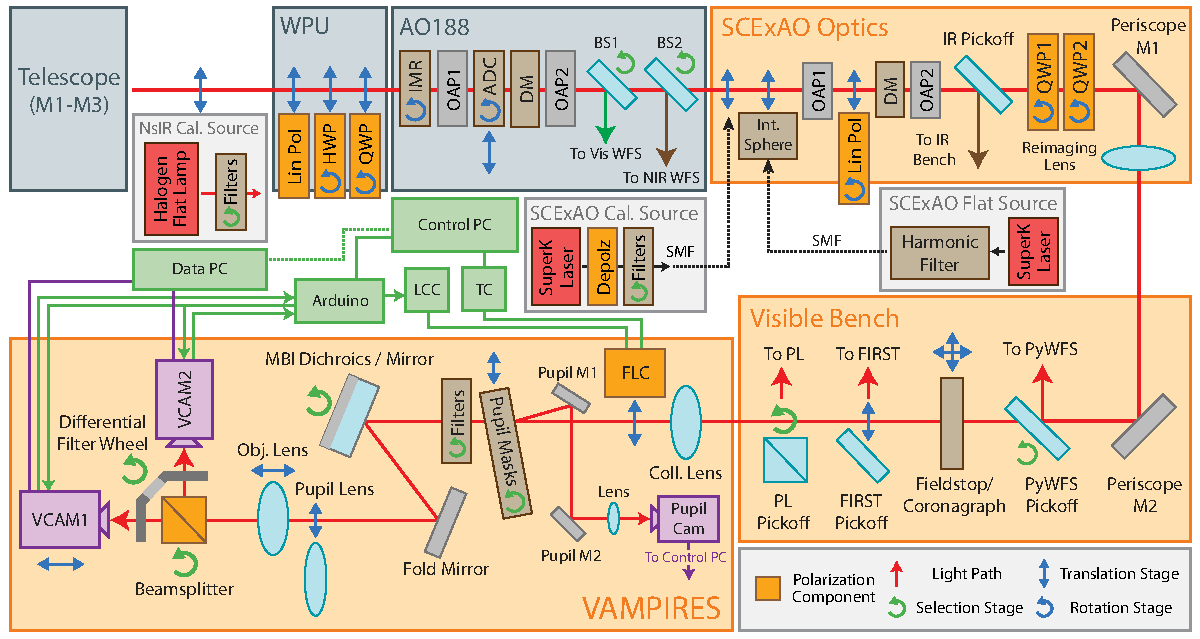
\includegraphics[width=\textwidth]{figures/VAMPIRES_diagram.pdf}
    \caption{VAMPIRES Instrument Schematic}
    \label{fig:schematic}
\end{figure*}

The Visible Aperture-Masking Polarimetric Imager/Interferometer for Resolving Exoplanetary Signatures (VAMPIRES) is the visible-light imager sub-instrument of the Subaru Coronagraphic Extreme Adaptive Optics testbed (SCExAO; \citet{jovanovic_subaru_2015}). SCExAO is a one-of-a-kind platform for high-contrast technological development and observations on the \SI{8.2}{\meter} Subaru telescope. SCExAO is mounted on the infrared Nasymth platform of Subaru behind the facility adaptive optics instrument, AO188 \citep{minowa_performance_2010}, which provides low-order correction with a curvature wavefront sensor to multiple instruments which are craned in and out of focus. AO188 also houses the K-mirror image rotator and atmospheric dispersion correcter (ADC).

The light from AO188 is split with a dichroic beamsplitter which transmits red to infrared light ($\lambda >$\SI{600}{\nano\meter}). This light enters SCExAO and is immediately collimated and corrected with a 2000-actuator Boston Micro Machines deformable mirror (DM), which has 45 actuators across the SCExAO pupil and operates at $\sim$\si{\kilo\hertz} speeds for extreme AO correction. Following the DM is a pupil mask which slightly undersizes the pupil (95\%, equivalent diameter of \SI{7.8}{\meter}) and blocks out two of the broken DM actuators. The beam is split with a near-IR dichroic filter ($\lambda=$\SI{950}{\nano\meter}), reflecting the visible light into a periscope which routes the beam onto a different optical bench and focuses the light with a reimaging lens.

Once the light is on the visible bench of SCExAO it encounters a series of pickoffs for routing the light to various modules of SCExAO. The first is the pickoff for the visible pyramid wavefront sensor (PyWFS), which has multiple filters for sending more or less light to the wavefront sensor to assure sufficient S/N during observations. Typically an \SI{800}{\nano\meter} dichroic filter is used, which effectively cuts off light below $\lambda <$\SI{775}{\nano\meter} due to its \ang{20} tilt. Then the light passes through a fieldstop that houses the suite of Lyot coronagraph masks (\autoref{sec:coronagraphy}) as well as a \SI{3}{\arcsecond}x\SI{3}{\arcsecond} fieldstop. After the fieldstop are two pickoffs for the fiber-fed instrument FIRST. These pickoffs typically use non-polarizing gray beamsplitters which allows simultaneous observations in VAMPIRES with appropriate focus shifts.

Finally, the remaining light (\SIrange{600}{775}{\nano\meter}) reaches the VAMPIRES collimating lens, after which is a deployable ferroelectric liquid crystal (FLC), a wheel for pupil-plane optics, and a standard filter wheel. The pupil wheel houses sparse aperture masks, neutral-density (ND) filters, and the coronagraph Lyot stops. This wheel is at $\sim$\ang{6} so that light reflected off the masks can be imaged by a separate pupil-viewing camera. The standard filter wheel houses five \SI{50}{\nano\meter}-wide bandpass filters for standard imaging as well as an empty slot for broadband observations, After this filter wheel is a separate baffle for the VAMPIRES fore-optics to reduce scattered light from motor encoders and electronic devices on the SCExAO bench. 

The beam then reaches a newly-developed multiband imaging (MBI) optic. This optic uses multiple dichroics with unique angles-of-incidence (AOI) to split broadband light into multiple fields imaged on the detector (\autoref{fig:mbi_schematic}). Our design uses three shortpass dichroic filters with a protected silver mirror at the back creating four $\sim$\SI{50}{\nano\meter} fields which roughly match the standard bandpass filters. This optic can be rotated \ang{180} to place a protected silver mirror in the beam, instead, creating a single image. In both cases, the light has a $\sim$\ang{10} reflection off a protected silver fold mirror before reaching the removable pupil-imaging lens and the objective lens.

\begin{figure}
    \centering
    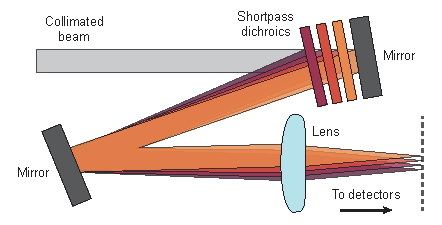
\includegraphics[width=\columnwidth]{figures/mbi_schematic.pdf}
    \caption{Schematic drawing for the multiband imaging dichroic principle. Broadband collimated light reaches the stack of dichroics plus mirror, each of which has a unique angle of incidence (AOI). The light reflected by each dichroic will have its own field in the focal plane due to the AOI. The light transmitted by each dichroic will pass onto the next optic, until all remaining light is reflected by a mirror at the back. of the stack.\label{fig:mbi_schematic}}
\end{figure}

As the light is focusing it passes through the beamsplitter wheel, which has a non-polarizing 50/50 beamsplitter cube, a wire-grid polarizing beamsplitter cube, or the light can be imaged without a beamsplitter onto a single detector, only. Because the beamsplitter cubes are \SI{25}{\milli\meter} thick, there is a significant focus shift which is accomadated by a translation stage on one of the cameras and the objective lens. The last optic before the detectors is a differential filter wheel which houses four narrowband filters. These filters come in pairs and are deployed so each pair is imaged simultaneously in front of both cameras. The filter wheel can switch which camera a respective filter is in front of with a \ang{180} rotation, which allows differential imaging to cancel out the non-common path aberrations between the two beams \citep{uyama_high-contrast_2020}.

\begin{deluxetable}{cl}
\tabletypesize{\footnotesize}
\tablehead{
    \colhead{Name} & 
    \colhead{Value(s)}
}
\tablecaption{VAMPIRES specifications.\label{tbl:specs}}
\startdata
Diff. Limit & \SI{16.5}{\mas} at \SI{625}{\nm}, \SI{20.1}{\mas} at \SI{760}{\nm}\\
FOV & \SI{3}{\arcsecond} x \SI{3}{\arcsecond} \\
Plate Scale & \SI{6}{\mas/px} \\
Coronagraph & CLC-2, CLC-3, CLC-5, CLC-7, DGVVC \\
SAM & 7-hole, 9-hole, 18-hole, Annulus, RAP \\
Pupil Masks & LyotStop, Mirror, ND1.0, ND2.5 \\
Filters & 625-50, 650-50, 675-50, 725-50, 750-50, 775-50, \\
& Open, MBI \\
NB Filters & H$\alpha$, H$\alpha$-Cont, SII, SII-Cont \\
Beamsplitter & PBS, NPBS, Open \\
Polarimetry & HWP + PBS, HWP + FLC + PBS \\
\enddata
\end{deluxetable}

\section{Detectors}\label{sec:detectors}

For our upgrades we deployed two custom-modified \textit{Hamamatsu ORCA-Quest} qCMOS detectors\footnote{\url{https://www.hamamatsu.com/us/en/product/cameras/qcmos-cameras/C15550-20UP.html}}. These detectors were chosen for their fast readout ($\sim$500 Hz at 512x512), low read noise ($\sim$ 0.2 - 0.4 $e^-$ RMS), and high dynamic range ($\sim$ 85 - 90 \si{\decibel}). We modified the cameras to be compatible with the telescope glycol cooling loop which keeps the detectors at \SIrange{-45}{-40}{\celsius} without creating turbulence in the instrument from air cooling.

The detectors have two primary readout modes: the full-speed ``FAST'' mode, and the slower, but more sensitive, ``SLOW'' mode. In ``SLOW'' mode the registers are able to use the reduced readout rate to reach $\sim$0.2 $e^-$ RMS read noise. In ``FAST'' mode there is an electronic shutter that allows detector integration times (DIT) of \SI{7.2}{\micro\second} - \SI{1800}{\second}. The ``SLOW`` mode the DIT are limited to $\sim >$\SI{50}{\milli\second} depending on the camera crop. Because the detectors have rolling-shutter readout, the framerate is limited by the number of rows read and the duty cycle and become very low at the shortest DITs. In addition, when synchronizing the two detectors together the external trigger mode reduces framerates and duty cycle, below 50\% in some scenarios.

We measured a photon transfer curve using a calibration flat field source for both detectors in both readout modes using a non-polarizing beamsplitter cube. We removed the fixed-pattern noise through frame-differencing before performing a linear fit between the average signal and the signal variance. From this fit we extract the gain in \si{\electron/\second}. We measure the readout noise from the standard deviation of a bias frame and convert to \si{\electron} with the gain. We observe that the full well is greater than the maximum bit-depth, so the detectors only saturate at $2^{16}$ \si{adu}. During commissioning we also took dark frames with the detector caps covered. For data with significant signal, we did a linear fit of the signal to the exposure time to get the average dark current. We report our results in \autoref{tbl:detectors}.


\begin{deluxetable}{cccccc}
\tablehead{
    \multirow{2}{*}{Cam} & 
    \multirow{2}{*}{Mode} & 
    \colhead{Gain} & 
    \colhead{RN} & 
    \colhead{DC} & 
    \colhead{DR} \\
     &
     &
    \colhead{(\si{\electron/\adu})} &
    \colhead{(\si{\electron})} &
    \colhead{(\si{\electron/\second/\pixel})} &
    \colhead{(\si{\decibel})}
}
\tablecaption{VAMPIRES detector characteristics. Dynamic range (DR) derived from max signal ($2^{16}$ \si{\adu}) in \si{\electron} divided by the readout noise.\label{tbl:detectors}}
\startdata
VCAM1 & FAST & 0.103 & 0.40 & \num{3.6e-3} & 85 \\
VCAM1 & SLOW & 0.105 & 0.25 & \num{3.6e-3} & 90 \\
VCAM2 & FAST & 0.103 & 0.40 & \num{3.6e-3} & 85 \\
VCAM2 & SLOW & 0.105 & 0.22 & \num{3.6e-3} & 90 \\
\enddata
\end{deluxetable}

Our detectors are some of the most sensitive available commercially today, and compared to electron-multiplication technologies the calibration and operation of the detectors is much simpler. In a 536 by 536 pixel window the fixed-pattern noise is $\sim$TODO\%, so we recommend flat-fielding to correct for the pixel-to-pixel gain variations. Bias frames are quite structured due to the CMOS architecture, so we also recommend bias or sky-background frames for subtracting the structured offset. Other than that, the detectors are virtually free of cosmetics so we only apply bad-pixel correction to long exposures for cosmic-ray rejection. In ``SLOW'' mode we are readout-noise-limited until DIT$>$\SI{13}{\second} at which point the detectors are limited by the shot-noise of the dark signal.
\section{Instrument Control}\label{sec:control}

SCExAO uses multiple computers for real time control and computation to keep latency low. The detectors are especially important to have dedicated resources because they can produce over \SI{20}{GB/s} \textit{each}. The detectors are both connected to the SCExAO data acquisition computer- the incoming data is treated as a continuous video stream which can be saved directly to FITS files as well as forwarded over TCP ports for access on the SCExAO real time control computer. The data acquisition computer manages metadata by combining the observatory-provided FITS headers with the SCExAO internal status, which uses a \texttt{redis} database hosted on a dedicated machine. Observing data and calibrations are transferred nightly to the Subaru STARS2 archive.

The devices for controlling VAMPIRES (filter wheels, translation stages, etc.) are connected to their own dedicated computer with the exception of a few common-path devices. The interface for these devices is written in python\footnote{\url{https://github.com/scexao-org/device_control}} which allows easy scripting. The devices have a command-line interface and are also routed through a network service that allows remote control from any of the SCExAO machines. The camera and FLC triggers are controlled with a high-speed micro-controller\footnote{\url{https://learn.adafruit.com/adafruit-metro-m4-express-featuring-atsamd51}} over USB. When triggering the FLC there is a delay every-other frame which is used to accurately deinterleave the two FLC states from the video stream. The VAMPIRES cameras each have custom viewers written in \texttt{PyGame} which allow high-speed (\SI{30}{fps}) image display and have bindings for instrument control. This makes tasks like coronagraph alignment simple by using keyboard shortcuts with the arrow keys.

\begin{figure}
    \centering
    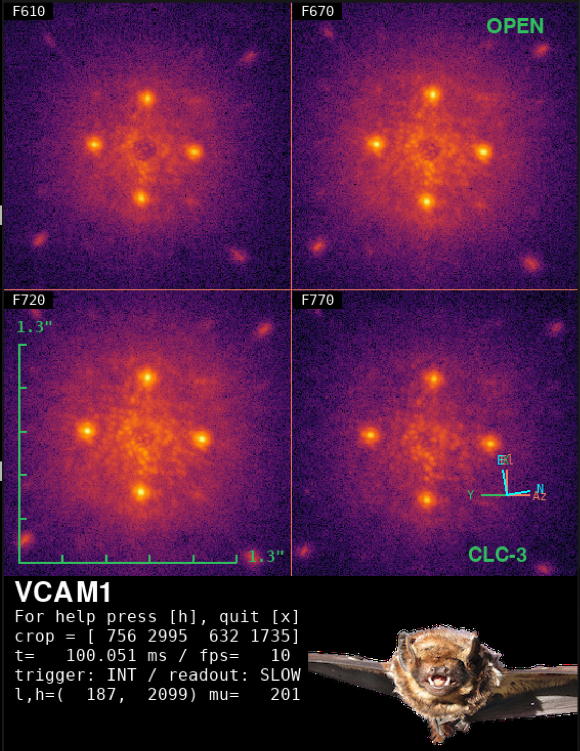
\includegraphics[width=0.95\columnwidth]{figures/vcam1_viewer.png}
    \caption{The custom \texttt{PyGame} camera viewer for VCAM1. Shown is a screenshot from on-sky observations on \formatdate{7}{7}{2023} in multiband imaging mode with the \SI{59}{\mas} coronagraph.}
    \label{fig:vcam1}
\end{figure}
% \tablenotetext{a}{The bat in the camera viewers is the Hawai`ian Ope`ape`a.}

\section{Filters and Instrument Throughput}\label{sec:filters}

VAMPIRES has five standard filters, four narrowband filters, an open broadband filter, the dichroic filters in the multiband optic, and two neutral density filters. The filter curves are compiled from manufacturer data and available openly. 

The Open filter is the widest and is constrained by the AO188 beamsplitter and the PyWFS pickoff. The standard filters are all \SI{50}{\nm}-wide bandpass filters, but the 775-50 bandpass is truncated due to overlap with the most commonly used PyWFS pickoff. The multiband filters come from consecutive transmissions/reflections through the stack of dichroics, and therefore the light transmitted through all filters will be more attenuated than the light reflecting off the first filter. The effective filter curves are $\sim$\SI{50}{\nm} wide and have minor leakage ($<$5\%) between some fields due to the imperfect dichroic transmissions. We also correct for the $\sim$\ang{10} AOI of the dichroic stack.

The narrowband filters are deployed in pairs for spectral differential imaging ($\Delta\lambda/\lambda=$\num{0.013}). The first pair of filters uses a \SI{1}{\nm} H$\alpha$ emission line filter with a \SI{2}{\nm} continuum filter, and the second uses a set of \SI{3}{\nm} SII doublet and continuum filters. All filter transmission curves are shown in \autoref{fig:filters} and summarized in \autoref{tbl:filters}.

\begin{figure}
    \centering
    \script{filter_curves.py}
    \includegraphics[width=\columnwidth]{figures/filter_curves.pdf}
    \caption{VAMPIRES filter transmission curves. All curves are normalized to the ``Open'' filter, which is the bandpass created from the dichroics upstream of VAMPIRES. The average wavelength for each filter is shown with a vertical dashed line.\label{fig:filters}}
\end{figure}

\subsection{Absolute Flux Calibration}

During commissioning spectrophotometric standard stars were observed in each filter with the non-polarizing beamsplitter. The standard spectra for each star was used for calibrating photometric zero points in \si{Jy} and \si{\electron/\second} as well as the instrument throughput. We used an empirical model for the atmospheric extinction \citep{buton_atmospheric_2013} which drives our uncertainties in absolute flux calibration. The filter calibration factors and zero points are summarized in \autoref{tbl:filters}.

The absolute flux calibration is summarized by the $C_{FD}$ coefficient, following \citet{gordon_james_2022}. This flux density conversion factor allows translation between data units and \si{Jy}. To use this factor the calibrated images need converted to instrumental flux with the gain and exposure time. Once in units of \si{\electron/s} apply the conversion factor to get to calibrated flux in \si{Jy}. To convert to surface brightness, divide by the area of a pixel (\SI{3.6e-5}{sq. arc/\pixel}). For Vega magnitudes, instead convert the corrected flux in \si{\electron/s} to instrumental magnitudes and correct with the appropriate zero point magnitude-
\begin{equation}
    m^\mathrm{filt}=\mathrm{ZP}_\mathrm{filt} - 2.5\log{\left(f\right)}
\end{equation}
or, equivalently-
\begin{equation}
    m^\mathrm{filt}=-2.5\log{\left(f/f_\mathrm{ZP}\right)}
\end{equation}
and to convert to surface brightness subtract the pixel area in square arcseconds converted to magnitudes-
\begin{equation}
    \Sigma^\mathrm{filt} = m^\mathrm{filt} - 2.5\log{\left(A_{px}\right)} = m^\mathrm{filt} + 11.1~\mathrm{mag/ sq.arc}
\end{equation}

These zero points and conversion factors are limited in their accuracy due to the ever-changing transmission from nightly variations in  atmospheric conditions and wavefront correction as well as telescope mirror coating degradation and dust build-up. For applications which require the highest photometric precision, doing \textit{in situ} photometry of an object or planning to observe a photometric standard with a calibrated spectrum at multiple airmasses will provide better accuracy than these values.


\begin{deluxetable}{ccccl}
\tablehead{
    \colhead{Object} &
    \colhead{Sp. Type} &
    \colhead{V (mag)} &
    \colhead{G (mag)} &
    \colhead{Ref.}
}
\tablecaption{Spectrophotometric standards used for photometric calibration. Both targets were observed on \formatdate{31}{08}{2023}.\label{tbl:specphot}}
\startdata
HD 15318 & B9III & 4.30 & \num{4.255+-0.004} & \\
HD 19445 & G2V & 8.06 & \num{7.904+-0.003} & \\
\enddata
\end{deluxetable}

\begin{deluxetable*}{ccccccccccccc}
\tablehead{
    \multirow{2}{*}{Filter} &
    \colhead{$\lambda_\mathrm{ave}$} &
    \colhead{$\lambda_\mathrm{min}$} &
    \colhead{$\lambda_\mathrm{max}$} &
    \colhead{FWHM} &
    \multirow{2}{*}{$\Delta\lambda/\lambda$} &
    \colhead{Inst. Trans.} &
    \colhead{$\mathrm{QE}_\mathrm{ave}$} &
    \multicolumn{3}{c}{Zero Point} &
    \colhead{$C_{FD}$} \\
    &
    \colhead{(\si{\nm})} &
    \colhead{(\si{\nm})} &
    \colhead{(\si{\nm})} &
    \colhead{(\si{\nm})} &
    &
    \colhead{(\%)} &
    \colhead{(\%)} &
    \colhead{(mag)} &
    \colhead{(\si{\electron/s})} &
    \colhead{(\si{Jy})} &
    \colhead{(\si{Jy.s/\electron})}
}
\tablecaption{VAMPIRES filter information. Minimum and maximum wavelengths represent 50\% relative throughput. Zero points, relative throughput, and conversion factors estimated from spectrophotometric standard observations on \formatdate{31}{8}{2023} and all assume no beamsplitter. Zero points in Vega magnitudes map to instrument flux in \si{\electron/s}.\label{tbl:filters}}
\startdata
Open & 680 & 580 & 776 & 196 & 0.30 & 6.4 & 67 & 25.7 & \num{1.9e10} & 3550 & \num{1.9e-7} \\
625-50 & 625 & 601 & 649 & 49 & 0.08 & 4.4 & 74 & 24.0 & \num{4.1e9} & 3440 & \num{8.4e-7} \\
675-50 & 675 & 651 & 699 & 49 & 0.07 & 8.0 & 67 & 24.4 & \num{5.6e9} & 2990 & \num{5.4e-7} \\
725-50 & 725 & 700 & 749 & 49 & 0.07 & 11 & 61 & 24.5 & \num{6.4e9} & 2800 & \num{4.4e-7} \\
750-50 & 748 & 724 & 776 & 48 & 0.06 & 10 & 58 & 24.3 & \num{5.4e9} & 2680 & \num{5.2e-7} \\
775-50 & 763 & 750 & 776 & 26 & 0.03 & 6.6 & 56 & 22.8 & \num{1.4e9} & 2610 & \num{2.0e-6} \\
\tableline
F610 & 614 & 580 & 645 & 65 & 0.11 & 3.1 & 76 & 23.8 & \num{3.3e9} & 3560 & \num{1.1e-6} \\
F670 & 670 & 646 & 695 & 49 & 0.07 & 7.0 & 67 & 24.1 & \num{4.4e9} & 3040 & \num{6.9e-7} \\
F720 & 721 & 696 & 745 & 50 & 0.07 & 9.0 & 61 & 24.4 & \num{6.0e9} & 2860 & \num{4.8e-7} \\
F760 & 761 & 746 & 776 & 30 & 0.04 & 6.0 & 57 & 23.6 & \num{2.7e9} & 5210 & \num{2.0e-6} \\
\tableline
H$\alpha$ & 656.3 & 655.9 & 656.7 & 0.8 & 0.0012 & 4.9 & 69 & & & & \num{3.8e-5} \\
H$\alpha$-Cont & 647.7 & 646.7 & 648.6 & 1.9 & 0.0029 & 5.4 & 70 & & & & \num{1.3e-5} \\
SII & 672.7 & 671.2 & 674.1 & 2.9 & 0.0043 & 8.6 & 67 & 21.4 & \num{3.6e8} & 3090 & \num{8.6e-6} \\
SII-Cont & 681.5 & 680.0 & 683.0 & 3.0 & 0.0044 & 8.5 & 66 & 21.3 & \num{3.4e8} & 3035 & \num{8.8e-6} \\
% 625-50\\
\enddata
\end{deluxetable*}
\section{Coronagraphy}\label{sec:coronagraphy}

As a high-contrast testbed SCExAO seeks to push wavefront control and coronagraphy to its limits. Currently VAMPIRES is equipped with four Lyot-style coronagraphs with various focal plane mask sizes and a new vector-vortex phase mask. The focal plane masks are mounted in a precise three-axis translation stage for fine alignment due to the lack of a dedicated tip-tilt mirror for VAMPIRES. The four Lyot-style focal plane masks were designed to be partially transmissive (design 0.1\%; actual 0.6\%) circular dots with inner working angles (IWA) corresponding to roughly two, three, five, and seven resolution elements (2, 3, 5, and 7 $\lambda/D$) in radius. The new double-grating vector vortex coronagraph (DGVVC; PI: Doelman, D.) was deployed in November 2023. This mask requires further testing before being made available for observers, especially given the polarizing effects of the liquid crystal grating in the mask.

\subsection{Focal-plane masks}

A new set of Lyot focal plane masks were made for VAMPIRES for our upgrades so that each mask has a \SI{3}{\arcsecond}x\SI{3}{\arcsecond} fieldstop. These masks were constructed the same as \citet{lucas_visible-light_2022}, however we note the measured IWAs have changed slightly compared to the previous coronagraph masks. Flat-field images of the four CLC masks are shown in \autoref{fig:clc_masks} and for the DGVVC in \autoref{fig:dgvvc_masks}. The DGVVC field shows a faint azimuthal structure when using the polarizing beamsplitter due to the polarization effects of the mask itself. These features mostly disappear when using the non-polarizing beamsplitter.

\begin{figure}
    \centering
    \script{clc_masks.py}
    \includegraphics{figures/clc_masks.pdf}
    \caption{Flat-field images of the classic Lyot coronagraph (CLC) focal plane masks cropped to the inner \ang{;;2} FOV. Dust particles on the front and rear faces of the optic blemish the field.\label{fig:clc_masks}}
\end{figure}

\begin{figure}
    \centering
    \script{dgvvc_masks.py}
    \includegraphics{figures/dgvvc_masks.pdf}
    \caption{Flat-field images of the double-grating vector vortex coronagraph (DGVVC) cropped to the inner \ang{;;2} FOV. The left image is with the polarizing beamsplitter (PBS)  which shows an azimuthal variation in intensity. (Right) with the non-polarizing beamsplitter (NPBS) the effect is reduced, but not completely. The limits have been clipped to emphasize the azimuthal pattern. The frames show the amplitude mask obscuring the central defect of the mask.\label{fig:dgvvc_masks}}
\end{figure}

The focal plane masks all suffer to some degree from dust features on the front and back surfaces. These features  are problematic due to the transmission losses localized around dust particles. Flat-fielding can mitigate these effects but is hard to do successfully with VAMPIRES because the coronagraph mask mount is moved to align to the star, rather than the other way around. A dedicated tip-tilt solution for VAMPIRES before the coronagraph would be preferred, but space constraints and restrictions due to the common path optics of the PyWFS make this practically difficult (\autoref{fig:cad}).

We measured the mask IWAs by rastering the SCExAO internal calibration source across the focal plane mask and measuring the photometric throughput. We convert the motion stage position to on-sky angle using plate scale of \SI{1.8}{\arcsecond\per\milli\meter} (Lozi~J. private communication). We measured the flux as the total sum of the full frame. We normalize the throughput to the peak flux of the PSF far from the mask and measure the IWA where this normalized throughput is 50\%. We plot the throughput curves and IWA in \autoref{fig:iwa} and summarize the results in \autoref{tbl:coronagraph}.

\begin{deluxetable}{lcc}
\tablehead{\colhead{Name} & \colhead{Radius (\si{\micron})} & \colhead{IWA (\si{\mas})}}
\tablecaption{VAMPIRES coronagraph mask specifications.\label{tbl:coronagraph}}
\startdata
CLC-2 & 46 & 37 \\
CLC-3 & 69 & 59 \\
CLC-5 & 116 & 105 \\
CLC-7 & 148 & 150 \\
DGVVC & 7 & 61 \\
\enddata
\tablecomments{The radius of the DGVVC is the radius of the amplitude mask obscuring the central defect in the phase mask.}
\end{deluxetable}

\begin{figure}
    \centering
    \script{iwa.py}
    \includegraphics{figures/coronagraph_iwa.pdf}
    \caption{Normalized off-axis throughput for the various coronagraph masks in VAMPIRES measured on \formatdate{17}{11}{2023}. The throughputs are normalized so the minimum flux is 0 and the maximum flux is 1. The inner working angle (IWA) is marked with vertical dotted lines at the point where the throughput reaches 50\%.\label{fig:iwa}}
\end{figure}

\subsection{Pupil masks}

VAMPIRES has three Lyot stop masks for rejecting the light diffracted by the coronagraphic focal plane mask. There is one Lyot stop with moderate throughput (66\%) which is described in \citet{lucas_visible-light_2022}. This mask is coated with gold for high reflectivity, aiding alignment with the pupil camera and for a future low-order wavefront sensor. Two new masks were laser-cut from metal foil sheets and deployed in January 2024 with alternate geometry in order to improve the throughput of the masks (PI: Walk, A.). We show them alongside the VAMPIRES pupil in \autoref{fig:pupil_masks}.

We measure the geometric throughput $T_\mathrm{geom}$ of each mask by finding the ratio of pupil flux with and without the mask. We used the pupil imaging lens in the Open filter for our analysis and took images with each mask. We dark subtract and then median collapse the pupil images and then binarize the data to 0 or 1 with a threshold to remove non-uniform pupil illumination from the fiber-fed calibration source. We measure the geometric throughput with the ratio of the sums of each binarized pupil image to the unobstructed pupil.

We also measure the photometric throughput for each mask by doing aperture photometry with our internal source in the Open filter. We used apertures with \SI{175}{\pixel} radius and a \SI{10}{\pixel} wide annulus from \SIrange{200}{210}{\pixel} for background subtraction and calculate the relative flux values (in \si{\electron/\second}). The photometric throughput is consistently lower than the geometric throughput, with a relative ratio of $T_{phot}=0.93\cdot T_{geom}$. The mask specifications and throughput measurements are listed in \autoref{tbl:pupil}.


\begin{figure}
    \centering
    \script{pupil_masks.py}
    \includegraphics{figures/pupil_masks.pdf}
    \caption{Images of the VAMPIRES pupil and coronagraphic pupil masks. (Top left) the VAMPIRES pupil without any masks. (Top right) the reference pupil laser-cut mask. (Bottom left) the laser-cut Lyot stop optimized for throughput. (Bottom right) the gold-plated Lyot stop from \citep{lucas_visible-light_2022}.\label{fig:pupil_masks}}
\end{figure}

\begin{deluxetable}{lcccccc}
\tabletypesize{\scriptsize}
\tablehead{\multirow{2}{*}{Name} & \multirow{2}{*}{Type} & \colhead{$D_\mathrm{in}$} & \colhead{$D_\mathrm{out}$} & \colhead{$w_s$} & \colhead{$T_{geom}$} & \colhead{$T_{phot}$}  \vspace{-0.75em}\\
    & & \colhead{(\si{mm})} & \colhead{(\si{mm})} & \colhead{(\si{\micron})} & \colhead{(\%)} & \colhead{(\%)}
}
\tablecaption{VAMPIRES Lyot stop specifications.\label{tbl:pupil}}
\startdata
Telescope Pupil & & \num{1300} & \num{7950} & & - & -\\
SCExAO Pupil & C & & 14 & & 100 & 100 \\
\tableline
LyotStop-S & M & 2.14 & 7.06 &  & 98.2 & 88.3 \\
LyotStop-M & M & 2.82 & 6.99 &  & 89.4 & 79.1 \\
LyotStop-L & G & 3.16 & 6.33 &  & 66.1 & 61.4 \\
\enddata
\tablecomments{The telescope pupil is the effective pupil at the Nasymth IR platform .The stop type is either ``G'' for the gold-plated glass window, ``M'' for the laser-cut metal sheet foil, or "C" for laser-cut carbon fiber sheets. The geometric throughput is measured using the pupil imaging lens and the internal source.}
\end{deluxetable}

\subsection{Coronagraphic point-spread function}

We show the coronagraphic PSF for all focal plane masks and all Lyot stops in \autoref{fig:bench_coro_profiles} using the Open filter and the SCExAO internal source.

\subsection{Calibration speckles}

VAMPIRES uses the SCExAO deformable mirror to create calibration speckles (``astrogrid'') for precise astrometry and photometry of the star behind the coronagraph mask \citep{sahoo_precision_2020}. The calibration speckles are typically configured to produce an ``X'' with separations of 10.3, 15.5, or 31.0 $\lambda/D$. The relative photometry of the calibration speckles were measured in multiband mode, for each of the above separations, and at different DM probe amplitudes. 

The relative flux is measured by taking the peaks of the convolved calibration speckles divided by the peak of the on-axis PSF. We fit bivariate quadratic functions of probe amplitude and wavelength to the relative PSF photometry (\autoref{eqn:astrogrid}). We note that these functions are only valid for a single astrogrid pattern due to the DM influence function and for DM amplitudes below 1 radian wavefront distortion ($\sim$\SI{95}{\nano\meter}). They also may vary with AO loop speed, but we do not characterize that here. We also fit the coefficients for the ``waffle'' spots passively created by the gridding of the DM. We report our model fits in \autoref{tbl:astrogrid}.
\begin{equation}
    \label{eqn:astrogrid}
    \frac{f_c}{f_*}\left( \lambda, A_{DM} | c \right) = c \cdot A_{DM}^2 / \lambda^2
\end{equation}


TODO READ RESULTSThe power law scaling fits well except for the brightest, closest calibration speckles.

To minimize the negative effects of astrogrid (namely photon noise in the control radius) the amplitude and separation should be tuned so the pattern is barely detectable. There is essentially a trade-off between centroid accuracy due to astrogrid S/N and contrast, and we recommend observers aiming for a speckle brightness a factor of a few above the PSF brightness at that separation. Using \autoref{fig:onsky_psf_profiles} this corresponds to roughly $<10^{-3}$ at 10$\lambda/D$ (\SI{7}{\nano\meter} astrogrid) and $<$\num{5e-4} at 15$\lambda/D$ (\SI{7}{\nano\meter} astrogrid).

There are some practical considerations for using astrogrid, though, especially when using VAMPIRES simultaneously with other modules of SCExAO. For example, when using SCExAO/CHARIS for PDI the Wollaston prism forces the use of the 10.3$\lambda/D$ separation grid so that the speckles all land within the FOV in broadband mode. Similarly, the speckle brightness in the near-infrared is fainter for a given pattern amplitude, which means you may have brighter speckles in VAMPIRES than desired to achieve satisfactory S/N in CHARIS. Lastly, there are the effects of chromaticity for wide filters (like the Open filter) and for the widely separated astrogrid patterns, which may lower the achievable astrometric or photometric precision.

\begin{deluxetable}{lcc}
\tabletypesize{\small}
\tablehead{\colhead{Pattern} & \colhead{Separation ($\lambda/D$)} & \colhead{c}}
\tablecaption{Astrogrid relative photometry flux scaling.\label{tbl:astrogrid}}
\startdata
XYgrid & 10.3 & \num{11.5\pm0.007}\\
XYgrid & 15.5 & \num{5.97\pm0.005}\\
XYgrid & 31.0 & \num{0.490\pm0.001}\\
\enddata
\tablecomments{Photometry measured using \SI{12}{\pixel}-radius apertures. Astrogrid applied using \SI{1}{\kilo\hertz} modulation speed.}
\end{deluxetable}

\begin{figure}
    \centering
    \script{astrogrid_photometry.py}
    \includegraphics{figures/astrogrid_photometry.pdf}
    \caption{Relative photometric flux of the astrogrid calibration speckles. Each plot corresponds to a different speckle pattern and each curve corresponds to a given pattern amplitude (in mechanical microns applied to the DM). \label{fig:astrogrid_photometry}}
\end{figure}


\subsection{On-sky contrast curves}

We have measured the surface brightness profiles and contrast curves for the CLC-3 and CLC-5 coronagraph masks. Data were obtained from observations of HD 102438 and GL 758 (HD 182488). The data were processed using dark subtraction and flat correction. The data were taken in the multiband-imaging mode so for each field the astrogrid calibration speckles were used to register the frame and we combined the coregistered and median-collapsed frames into a spectral cube. We use the aperture photometry of the calibration speckles for flux conversion to contrast using the relative scaling factors (\autoref{eqn:astrogrid},\autoref{tbl:astrogrid}).

The surface brightness profiles are plotted in TODO. We used TODO algorithm for modeling the PSF for each wavelength. The 1$\sigma$ small-sample statistics corrected contrast curves \citep{mawet_fundamental_2014} are plotted in TODO. We also calculate the double-SDI contrast curve after radially scaling each field by its wavelength and subtracting the median frame before rescaling and collapsing.

\subsection{Residual atmospheric dispersion}

There is only a single broadband atmospheric dispersion corrector (ADC) in the common path of VAMPIRES. This can result in residual atmospheric dispersion, depending on the airmass. Residual dispersion can be seen as a shift in the PSF over different wavelengths range. When using a fixed coronagraph, this can cause the stellar PSF to actually appear only partially covered by the coronagraph mask. This is often seen in the K-band of coronagraphic low-dispersion CHARIS observations. With multiband imaging we can see this effect (\autoref{fig:resid_adc}), but it only affected the CLC-3 mask at airmasses above $\sim$\num{2.2} ($<$\ang{27} elevation). The larger masks (CLC-5 and CLC-7) would be less affected by the dispersion, but at a loss of inner working angle.

\begin{figure}
    \centering
    \script{resid_adc.py}
    \includegraphics{figures/resid_adc.pdf}
    \caption{Coronagraphic multiband imaging of HD163296 with the CLC-3 coronagraph at 2.25 airmass (\ang{26.3} elevation). The filter is labeled in the top left, the location of the star is marked with a cross, and the telescope elevation and azimuth axes are displayed with a compass in the bottom left. The image is shown with a square-root stretch with separate limits for each filter.\label{fig:resid_adc}}
\end{figure}

\subsection{Redundant apodizing pupil}

A redundant apodized pupil mask (RAP; PI: Leboulleux, L.) was deployed on VAMPIRES in September 2023. This mask apodizes the pupil in a way which creates a static dark hole that is robust to low-wind effect up to $\sim$\SI{1}{rad} RMS wavefront error. The trade-off is the limited inner and outer working angles and the fact that there is no attenuation of the stellar PSF, which may lead to saturation. We show the RAP mask, PSF, and profile from bench tests in the Open filter in \autoref{fig:rap}. Further testing on-sky is required before opening to observers and is future work.

\begin{figure}
    \centering
    \script{rap.py}
    \includegraphics{figures/rap.pdf}
    \caption{The redundant apodized pupil (RAP) mask. (Top left) a pupil image of the mask showing the apodization pattern. (Top right) a \ang{;;2}x\ang{;;2} FOV of the PSF produced by the RAP using the SCExAO internal source in the Open filter. The image is stretched to emphasize the dark hole from approximately \ang{;;0.1} to \ang{;;0.8}. (Bottom) a normalized radial profile of the top right PSF in log scale.\label{fig:rap}}
\end{figure}
\section{Polarimetry}\label{sec:polarimetry}

VAMPIRES is capable of polarimetry through the use of a broadband half-wave plate (HWP) and a wire-grid polarizing beamsplitter cube. This puts orthogonal polarization states on each detector which can be subtracted to measure linear polarization \citep{kuhn_imaging_2001}. To measure the two linear Stokes quantities ($Q$ and $U$) we modulate the HWP at angles \ang{0}, \ang{45}, \ang{22.5}, \ang{67.5}, allowing double-differencing to remove a significant portion of instrumental polarization.

For observations with DIT $<$ \SI{1}{\second} a fast achromatic ferro-electric liquid crystal (FLC) device can be inserted into the beam and synchronously modulated with every exposure. In this mode we can more effectively subtract the signals from fast-moving speckles by triple-differencing with the FLC modulation \citep{norris_vampires_2015}. VAMPIRES also uses two quarter-wave plates (QWP) for correcting the static instrumental birefringence, in particular from the periscope in SCExAO.

Polarimetric measurements are limited by instrumental polarization due to the many inclined surfaces and reflections in the common path of VAMPIRES. It is a well-established technique to model and remove the instrumental effects using Mueller calculus \citep{holstein_polarimetric_2020,joost_t_hart_full_2021}. For VAMPIRES we use internal calibrations with a halogen flat lamp and linear polarizer after the telescope M3 as a polarized source. We modulate the facility HWP and image rotator and create sum and difference images from both detectors in order to fit our Mueller matrix model for each VAMPIRES filter.  These calibrations are set up to be highly-automated using the python control code. 

\subsection{Polarimetric Spectral Differential Imaging}

We have developed a new mode for VAMPIRES for polarimetric measurements in the narrowband filters. Because the narrowband filters are stored in the differential filter wheel only one camera receives light from the filter. To enable polarimetry we must switch the differential filter between the cameras for each HWP position so that we measure both horizontal and vertically polarized light for each filter. In post-processing one can choose to do standard double- or triple-differencing separately for each filter to get the Stokes data, or the two filters can be subtracted immediately before differencing for spectral differential imaging (SDI).

Polarimetric SDI (PSDI) will allow direct measurement of the polarized fraction of narrowband emission, which is particularly interesting for H$\alpha$ imaging of circumstellar disks. For example, the H$\alpha$ emission around AB Aur may be from a forming protoplanet \citep{currie_images_2022}, in which case the emission should be unpolarized. If the H$\alpha$ emission is polarized this points to different hypothesis, such as stellar emission scattering off dust grains \citep{zhou_uv-optical_2023}. This technique has been tested with an internal calibration source and future observations will be used to demonstrate our method on-sky.
\section{First Light Results}\label{sec:firstlight}

The VAMPIRES upgrades were tested on-sky from June to August 2023, some results from our first-light observations are presented below.

\subsection{HD 169142\label{sec:hd169142}}

We observed the young star \textit{HD 169142}, which is a known protoplanetary disk host, on \formatdate{7}{7}{2023}. We used the multiband imaging mode without the FLC (slow polarimetry mode) with the \SI{105}{\mas} Lyot coronagraph for \SI{55}{minutes}, resulting in \SI{47}{minutes} of data- roughly an \SI{85}{\%} observing efficiency. We reduced this data as described in \autoref{sec:processing} with background subtraction and double-difference polarimetric reduction with an idealized Mueller-matrix correction. We used an annulus from \ang{;;0.24} to \ang{;;0.33} for removing residual instrumental polarization since this matches the expected region of the cavity of the disk \citep{bertrang_hd_2018}. We convert the data from \si{adu} to \si{mJy/arcsec^2} using a synthetic photometry of a standard F2V model spectrum \citep{pickles_stellar_1998} normalized to i=\SI{7.978}{mag} \citep{zacharias_fourth_2013}. We note that using an idealized Mueller matrix is not optimal, but future analysis will be done when the upgraded instrument polarization calibration is completed.

The $Q_\phi$ frames from each filter, which we use to represent the polarized intensity, are shown in \autoref{fig:hd169142_mosaic}. The inner disk is visible at all wavelengths. We also show a version scaled by the squared stellocentric distance to normalize the stellar irradiation. The scaled version shows the large disk gap and the inner rim of the outer disk. We note that compared to images from \cite{bertrang_hd_2018} we have worse S/N and do not fully resolve the outer disk. However, our observations have smaller spectral bandwidth per image and use a fraction of the detector integration time (\SI{1}{s} versus \SIrange{6}{10}{s}). Future observations with longer detector integration times are needed to resolve the full disk structure.

\begin{figure*}[t]
    \centering
    \script{HD169142.py}
    \includegraphics[width=\textwidth]{figures/20230707_HD169142_Qphi_mosaic.pdf}
    \caption{\formatdate{7}{7}{2023} VAMPIRES observations of \textit{HD 169142} in multiband imaging mode. Each column represents one multiband filter. The top row is the Stokes $Q_\phi$ image in linear scale (different scale for each filter). The bottom row is  Stokes $Q_\phi\times r^2$, where $r$ is the stellocentric distance to normalize the stellar irradiation (different scale for each filter). All data are rotated so that North is up and East is to the left.\label{fig:hd169142_mosaic}}
\end{figure*}

We take each $Q_\phi$ frame and integrate the flux out to \ang{;;1} and compare to the same flux value measured in the Stokes I frame. The relative fluxes for each filter are shown in \autoref{fig:hd169142_flux}. The mean integrated partial-polarization of the disk, \SI{0.6}{\%}, roughly matches the expectations given similar measurements from TODO and TODO. 

\begin{figure}
    \centering
    \script{HD169142.py}
    \includegraphics[width=\columnwidth]{figures/20230707_HD169142_Qphi_flux.pdf}
    \caption{\formatdate{7}{7}{2023} VAMPIRES \textit{HD 169142} radial profiles for the polarized intensity (top; taken from $Q_\phi$ frame) and fractional polarized flux (bottom; $Q_\phi/I$). The profiles are taken with annuli of a width of 4 pixels starting from the coronagraph IWA (\si{105}{mas}). The region of inner disk shows clearly that the dust scatters more at redder wavelengths.\label{fig:hd169142_flux}}
\end{figure}

In future work we plan to model and fit geometric disk profiles to analyze the scattering geometry of this disk, allowing a measurement of the scattering phase function of the dust at multiple wavelengths. These measurements give us color information about the scattering properties of the dust which normally requires multiple observations for each filter, but we obtain them in a one observing sequence by using the multiband imaging technique.

\subsection{R Aqr\label{sec:raqr}}

We performed narrowband H$\alpha$ observations of the Mira variable \textit{R Aqr} on \formatdate{7}{7}{2023} with VAMPIRES. We decided to slightly increase our observing efficiency by not switching the differential filters between each camera- we were not concerned with non-common path aberrations for this short demonstration sequence.

For each camera (and therefore each narrowband filter) we reduced the data following \autoref{sec:processing} with dark subtraction and phase cross-correlation centroiding. We derotate all images to north up east left before coadding with a pixel-by-pixel median. We use calibration factors from \autoref{tbl:filters} and the detector gain and exposure time to convert data from \si{adu} into units of \si{mJy/arcsec^2}. The collapsed images are shown in \autoref{fig:raqr}.

\begin{figure}
    \centering
    \script{RAqr.py}
    \includegraphics[width=\columnwidth]{figures/20230707_RAqr_Halpha.pdf}
    \caption{\formatdate{28}{6}{2023} VAMPIRES \textit{R Aqr} reduced H$\alpha$ filter image with logarithmic stretch showing the emission nebula.\label{fig:raqr}}
\end{figure}

\begin{figure}
    \centering
    \script{RAqr.py}
    \includegraphics[width=\columnwidth]{figures/20230707_RAqr_mosaic.pdf}
    \caption{\formatdate{28}{6}{2023} VAMPIRES \textit{R Aqr} Reduced images in linear stretch. Both images are in units of \si{mJy/arcsec^2} and have the same limits. (left) The H$\alpha$ image showing the giant star and a bright emission clump to the northeast. (right) The H$\alpha$-continuum image which only contains emission from the giant star.\label{fig:raqr_mosaic}}
\end{figure}

\subsection{Neptune\label{sec:neptune}}

We observed gas giant \textit{Neptune} on \formatdate{11}{7}{2023} in the multiband imaging mode to test VAMPIRES capabilities for planetary astromony. \textit{Neptune} was a good target due to its angular diameter being within the VAMPIRES FOV ($<$\ang{;;3}) and without being too faint. The adaptive optics systems during this observation were not able to correct for wavefront errors with the typical performance due to the lack of a point-source guide star- rather using the extended planet itself as a guide star. In addition, this data requires slight modifications in the post-processing to address the unique features of a planetary image. The adopted planetary information for these observations is shown in \autoref{tbl:neptune}

\begin{deluxetable}{cl}
\tablehead{
    \colhead{Parameter} &
    \colhead{Value}
}
\tablecaption{Planetary parameters for Neptune adopted in this study from JPL horizons DE441 ephemerides.\label{tbl:neptune}}
\startdata
Apparent diameter & \ang{;;2.313102} \\
North pole angle & \ang{318.0816} \\
North pole distance & \ang{;;-1.058}
\enddata
\tablereferences{\url{https://ssd.jpl.nasa.gov/horizons/}}
\end{deluxetable}


For processing, we attempted flat-field correction with some success. Multiband observations are uniquely difficult to flat field, because a single detector image has four images at different wavelengths, and therefore different intensities when illuminated with a calibration laser or flat lamp. We developed a simple computer-vision algorithm to fit rotated rectangles to each flat-field and normalizes each field with a local value. Unfortunately, in this data there was a bug in the data acquisition software which truncated all data to 15-bit unsigned integers, artificially saturating readout values greater than $2^{15}$. This has been fixed, but our calibration flats for the F720 filter from this epoch all suffer from this truncation leading to flat-field errors (as can be seen in \autoref{fig:neptune_mosaic}). We also discovered some imperfect flat-field correction of some dust features in other fields, likely due to small differences in the optical alignment of the glass fieldstop.

We did not attempt to centroid this data, instead we registered each frame using the field positions fit during our flat-field procedure. Future work would benefit from more precise centroiding, perhaps using a radon transform to fit the disk position for each image. We use calibration factors from \autoref{tbl:filters} and the detector gain and exposure time to convert data from \si{adu} into units of \si{Jy/arcsec^2}. Similar to \autoref{sec:hd169142} we perform double-difference polarimetric reduction with an idealized Mueller-matrix correction. \citet{schmid_limb_2006} notes that the disk integrated $Q/I$ and $U/I$ frames for Neptune are effectively zero within systematic errors due to its radially-symmetric limb polarization, so we used an aperture the size of the planet for instrument polarization measurement and correction. We derotate all Stokes images to north up and east left before combining with a pixel-by-pixel median. We noticed in this data that the Stokes Q and U frames do not perfectly align with the expected \ang{45} and \ang{0} nulls, respectively- especially at shorter wavelengths (F620, F670). We assume this is due to imperfect modeling of the instrumental polarization effects in the Mueller-matrix model, which is left to future work., Interestingly, we do not see this same effect for the disk observations of \autoref{sec:hd169142}.

We calculate an alternative set of radial Stokes parameters, $Q_r$ and $U_r$, following \citet{schmid_limb_2006},
\begin{align}
    Q_r &= Q\cos{\left(2\theta\right)} + U\sin{\left(2\theta\right)} \\
    U_r &= -Q\sin{\left(2\theta\right)} + U\cos{\left(2\theta\right)}
\end{align}
For an optically thick planetary atmosphere like Neptune's, the most probable alignment of the electric field is radially (as opposed to azimuthally for \autoref{eqn:radial_stokes}), which makes $Q_r$ approximately equal to the polarized intensity. We expect $U_r$ to be minimized, at least to first order, and we attempt to correct residual polarization errors in our data by offsetting the angle, $\theta$, for the radial Stokes parameters in each filter. The required angle offset for each filter was \ang{21.3}, \ang{5.6}, \ang{0.3}, and \ang{1.0}, respectively.

We show the corrected radial Stokes $Q_r$ frames and Stokes $I$ frames in \autoref{fig:neptune_mosaic}. We see clear limb polarization in all filters with little polarization in the center of the image and the maximum polarization at the edge. We see roughly equal polarization along the whole limb (as opposed to concentration at the poles or equator). We plot radial profiles of the $Q_r$, $I$, and $Q_r/I$ for each filter in \autoref{fig:neptune_flux}. The total intensity frames show some signs of a polar cloud along with some mild banding structures, especially in the F720 frame (disregarding any flat-field errors).

\begin{figure*}[t]
    \centering
    \script{neptune.py}
    \includegraphics[width=\textwidth]{figures/20230711_Neptune_mosaic.pdf}
    \caption{\formatdate{11}{7}{2023} VAMPIRES observations of \textit{Neptune} in multiband imaging mode. Each column represents one multiband filter. All data are rotated so that north is up and east is to the left. The top row is the Stokes $Q_r$ image in linear scale (different scale for each filter). The bottom row is Stokes $I$ (different scale for each filter). The apparent diameter of the disk is shown with a circle and the southern polar axis is designated with a line (based on JPL horizons ephemerides). Note there are spurious features in the total intensity images due to flat-field errors (dust, etc.). \label{fig:neptune_mosaic}}
\end{figure*}

\begin{figure}[t]
    \centering
    \script{neptune.py}
    \includegraphics[width=\columnwidth]{figures/20230711_Neptune_flux.pdf}
    \caption{Radial profiles of polarimetric observations of Neptune. All profiles use apertures 10 pixels wide. (top) total intensity. (middle) radial stokes intensity. (bottom) the flux-weighted, \label{fig:neptune_flux}}
\end{figure}

\section{Conclusions}\label{sec:conclusions}


\begin{acknowledgements}
We wish to recognize and acknowledge the significant cultural role and reverence that the summit of Maunakea has always had within the indigenous Hawaiian community. We are grateful and thank the community for the privilege to conduct observations from this mountain.

We thank Joshua Hacko (NH Micro), Iven Hamilton (UH), Shane Jacobson (UH/Gemini), Michael Lemmin (NAOJ), Paul Sumner (Optiline), Lucio Ramos (NAOJ), Paul Toyoma (UH), and Matthew Wung (NAOJ) for their time and expertise in the manufacturing, assembly, testing, and integration of the VAMPIRES upgrades.

We thank Timothy Brandt and collaborators for the use of data obtained under Subaru proposal IDs o23149 and o23286. We thank Michael Fitzgerald and collaborators for the use of data obtained under Subaru proposal ID o23150. We thank telescope operators Larissa Shumacher, Erin Dailey, Andrew Neugarten, Aidan Walk, TODO for their support for the observations used in this work.
\end{acknowledgements}
\facility{Subaru (SCExAO)}
\software{}

\bibliography{bib}

\appendix
\section{Observing Log\label{sec:log}}

In \autoref{tbl:obslog} we list all observations used for this work. 


\begin{deluxetable*}{cccccccccccc}
\tablehead{
    \colhead{Date (UTC)} &
    \colhead{Object} &
    \colhead{Obs. Mode} &
    \colhead{Filter} &
    \colhead{Pol. Mode} &
    \colhead{Coron.} &
    \colhead{DIT (s)} &
    \colhead{$N_\mathrm{Exp}$} &
    \colhead{$T$ (min)} &
    \colhead{PI} &
    \colhead{Obs. ID}
}
\tablecaption{Observing log\label{tbl:obslog}}
\startdata
2023/06/27 & HD 222800 & IMAG\_SDI & H$\alpha$/H$\alpha$-Cont &  & & & & & Engineering & o23013 \\
2023/06/29 & HD 102438 & IMAG\_MBI & MBI &  & CLC-5 & & & & Brandt, T. & o23149 \\
2023/07/07 & HD 169142 & IPOL\_MBI & MBI & Slow & CLC-5 & & & & Lucas, M. & o23166 \\
2023/07/10 & & &  & &   && & & Lucas, M. & o23161 \\
2023/08/31 & HD 15318 & IMAG & 625-50 & & & & & & Engineering & o23013 \\
2023/08/31 & HD 15318 & IMAG & 675-50 & & & & & & Engineering & o23013 \\
2023/08/31 & HD 15318 & IMAG & 725-50 & & & & & & Engineering & o23013 \\
2023/08/31 & HD 15318 & IMAG & 750-50 & & & & & & Engineering & o23013 \\
2023/08/31 & HD 15318 & IMAG & 775-50 & & & & & & Engineering & o23013 \\
2023/08/31 & HD 15318 & IMAG & Open & & & & & & Engineering & o23013 \\
2023/08/31 & HD 15318 & IMAG\_MBI & MBI & & & & & & Engineering & o23013 \\
2023/08/31 & HD 15318 & IMAG\_SDI & SII/SII-Cont & & & & & & Engineering & o23013 \\
2023/08/31 & HD 15318 & IMAG\_SDI & H$\alpha$/H$\alpha$-Cont & & & & & & Engineering & o23013 \\
2023/08/31 & HD 19445 & IMAG\_SDI & H$\alpha$/H$\alpha$-Cont & & & & & & Engineering & o23013 \\
2023/09/01 & HD 182488 & IMAG\_MBI & MBI & & CLC-5 & & & & Brandt, T. & o23286 \\
\enddata
\end{deluxetable*}
\section{Instrument models\label{sec:models}}

A CAD model of VAMPIRES on the visible bench of SCExAO is shown in \autoref{fig:cad}


\begin{figure*}
    \centering
    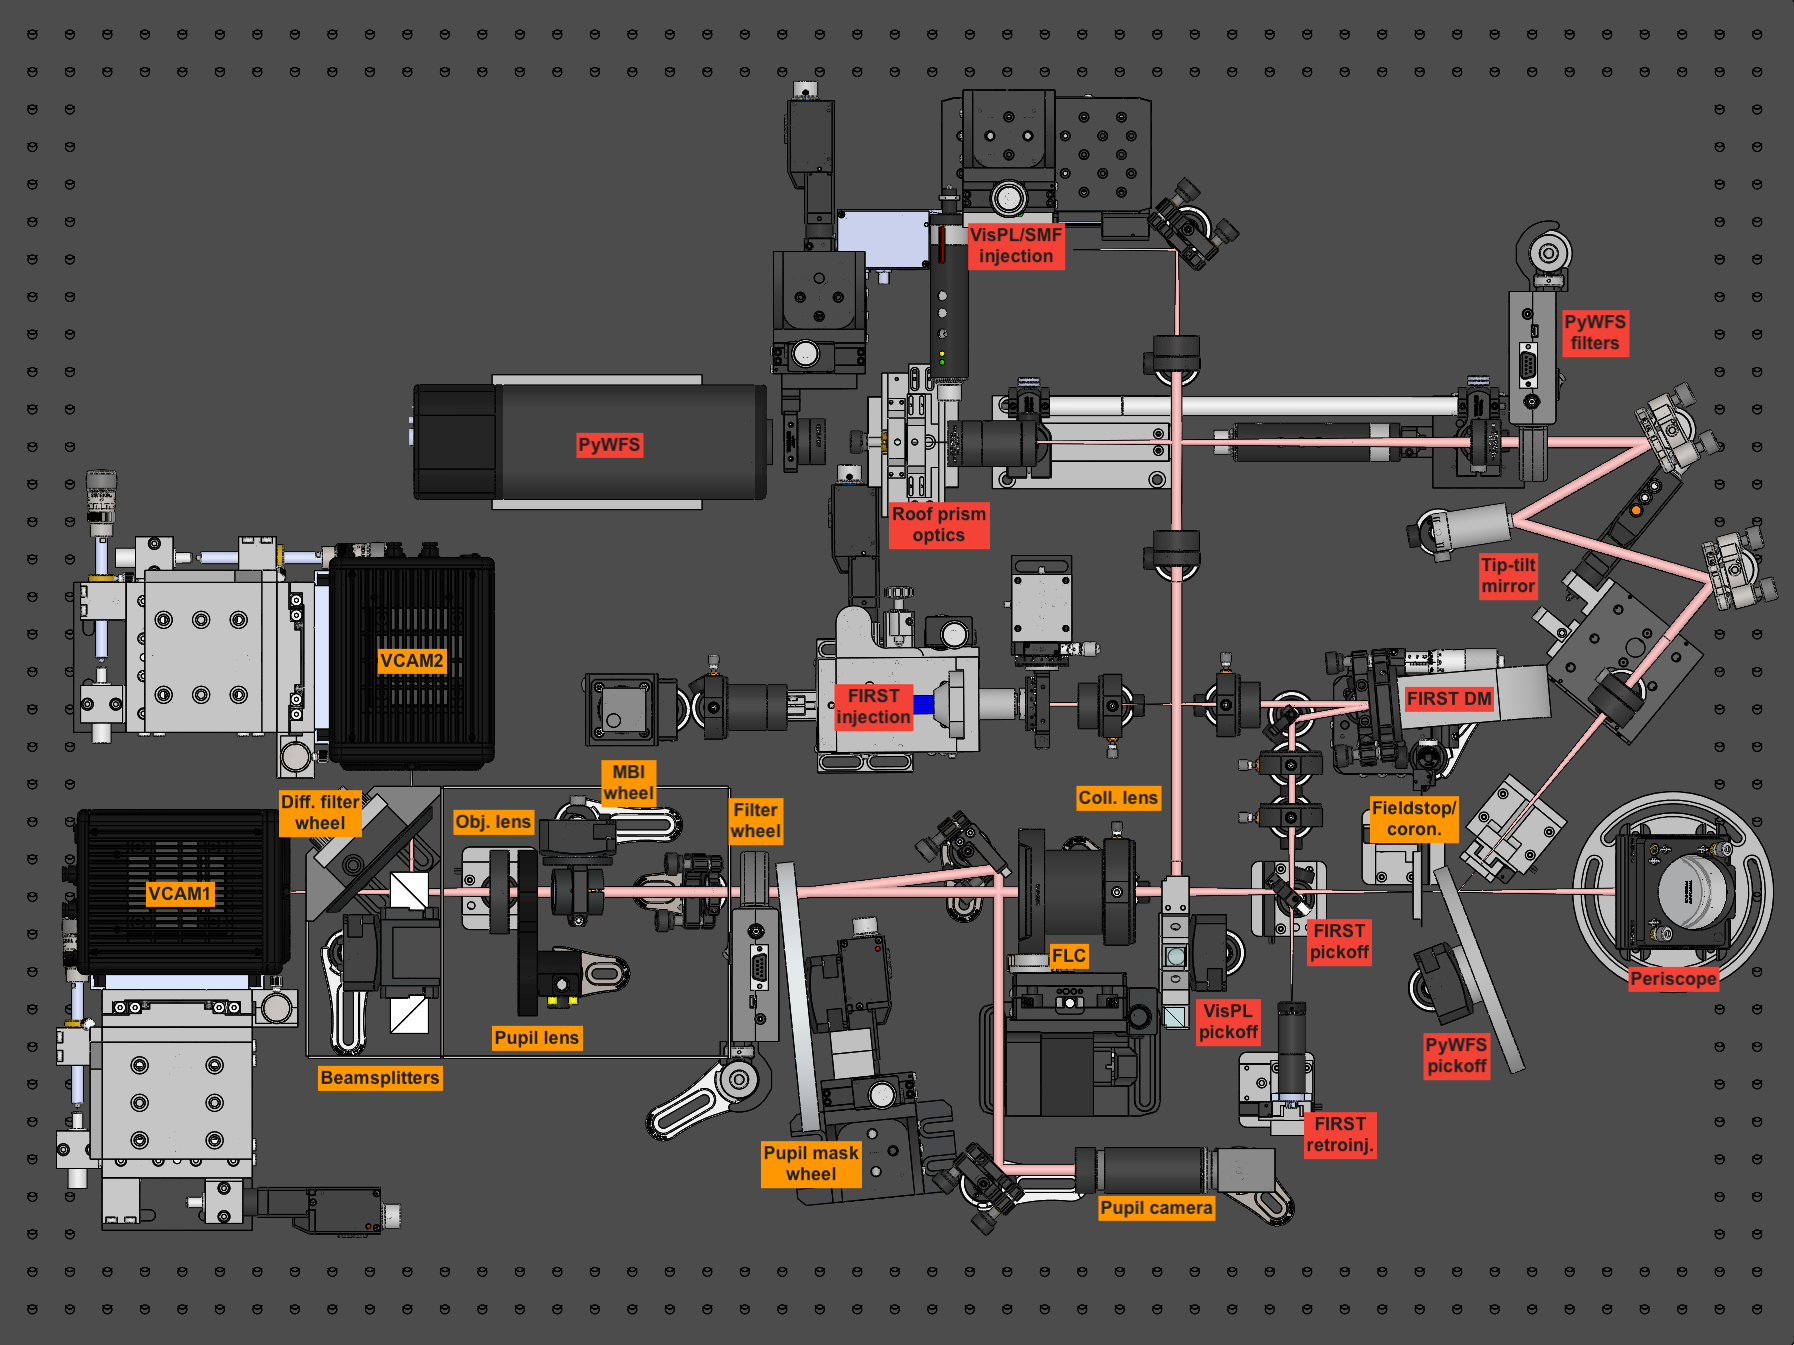
\includegraphics[width=\textwidth]{figures/visible_bench_annotated.png}
    \caption{SCExAO visible bench including the PyWFS, FIRST injection, and VAMPIRES. VAMPIRES optics are labeled in orange and FIRST/PyWFS optics are labeled in red. The total size of the optical table shown is \SI{120}{\cm} by \SI{90}{\cm}. Parts of the baffling around VAMPIRES optics as well as the optical bench enclosure are hidden for clarity.\label{fig:cad}}
\end{figure*}


\section{Data and Code Availability}
This study was carried out using the reproducibility software \href{https://github.com/showyourwork/showyourwork}{\showyourwork} \citep{luger_mapping_2021}, which leverages continuous integration to programmatically create the figures and compile this manuscript. Each figure caption contains a link to the script used to make the figure (at the commit corresponding to the current build of the manuscript). The git repository associated to this study is publicly available at \url{\GitHubURL}.

\end{document}
